
%%%%%%%%%%%%%%%%%%% -------- INICI DOCUMENT ---------%%%%%%%%%%%%%%%%%%%%%%%%
\documentclass[10pt]{book}

% mis paquetes
\usepackage[utf8]{inputenc} % Para codificar el archivo con UTF-8
\usepackage[english]{babel} % Para usar la traducción española
\usepackage[margin=1.5in]{geometry} % Para definir los márgenes del documento
\usepackage{amsmath} % Para utilizar simbolos matemáticos
\usepackage{amsfonts} % Para utilizar diferentes fuentes matemáticas
\usepackage{amsthm} % Para crear teoremas y definiciones matemáticas
\usepackage{amssymb} % Para utilizar símbolos matemáticos adicionales
\usepackage{graphicx} % Para incluir imágenes en el documento
\usepackage[usenames,dvipsnames]{xcolor} % Para utilizar diferentes colores
\usepackage{float} % Para definir flotantes (imágenes, tablas, etc.)
\usepackage[siunitx]{circuitikz} % Para crear diagramas de circuitos
\usepackage{tikz} % Para dibujar gráficos y diagramas
\usepackage{hyperref} % Para hacer enlaces hipervínculos en el documento
%\usepackage[numbers, square]{natbib} % Para crear bibliografías
\usepackage{fancybox} % Para crear cajas con bordes y fondos
\usepackage{epsfig} % Para incluir imágenes en formato EPS
\usepackage{soul} % Para resaltar texto con un fondo de color
\usepackage[framemethod=tikz]{mdframed} % Para crear marcos con bordes y fondos
\usepackage[colorinlistoftodos, color=orange!50]{todonotes} % Para agregar notas a tareas pendientes
\usepackage[framed,numbered,autolinebreaks,useliterate]{mcode} % Para incluir código en el documento
\usepackage[shortlabels]{enumitem} % Para personalizar listas enumeradas
\usepackage[version=4]{mhchem} % Para escribir fórmulas químicas
\usepackage{listings} % Para incluir código fuente en el documento
\usepackage{color} % Para personalizar los colores en el documento
\definecolor{mygreen}{RGB}{28,172,0} % Definir un color verde personalizado
\definecolor{mylilas}{RGB}{170,55,241} % Definir un color lila personalizado
\usepackage{subcaption} % Para crear subfiguras
\usepackage{url} % Para crear enlaces a páginas web
\usepackage{minted} % Para incluir código resaltado
\usepackage{wrapfig} % Para envolver texto alrededor de imágenes o figuras para crear una figura que "envuelve" el texto alrededor de ella.

\usepackage{siunitx}
\usepackage{vmargin}
\usepackage{layout}
\usepackage{fancyhdr}
\usepackage{vmargin}
\usepackage{setspace}
\usepackage{parskip}
\usepackage{caption} 
\usepackage[style=iso-numeric]{biblatex} %Bibliografia
\usepackage[final]{microtype}

\usepackage[style=iso-numeric]{biblatex}
\addbibresource{bibliography.bib}
\usepackage{tocloft}  % para list of equations

\newcommand{\listequationsname}{List of Equations}
\newlistof{myequations}{equ}{\listequationsname}
\newcommand{\myequations}[1]{%
    \addcontentsline{equ}{myequations}{\protect\numberline{\theequation}#1}\par}

\usepackage{bm} % bold math
\usepackage{acronym}
\usepackage[bottom]{footmisc}


%%%%%%%%%%%%%%%% DEFINICION DEL ESQUEMA DE COLORES DE PYTHON
%\usepackage{minted}
%\usepackage{xcolor} % to access the named colour LightGray
%\definecolor{LightGray}{gray}{0.9}
\usepackage{ulem} 
\usepackage{minted,xcolor}
\usemintedstyle{tango} %monokai
\definecolor{bg}{HTML}{E7E7E7} % from https://github.com/kevinsawicki/monokai

\lstset{
breakatwhitespace=false,	% sets if automatic breaks should only happen at whitespace
breaklines=true,	% sets automatic line breaking
frame=single,	% adds a frame around the code
numbers=left,	% where to put the line-numbers; possible values are (none, left, right)
showspaces=false,               % show spaces everywhere adding particular underscores; it overrides 'showstringspaces'
basicstyle=\small\ttfamily}
%\setlength{\parindent}{0cm}

%%%%%%%%%%%%%%%%%%%%%%%%%%%%%%%%%%%%%%%%%%%%%%%%%%%%%%%
%   _____ _    _  _____ _______ ____  __  __ 
%  / ____| |  | |/ ____|__   __/ __ \|  \/  |
% | |    | |  | | (___    | | | |  | | \  / |
% | |    | |  | |\___ \   | | | |  | | |\/| |
% | |____| |__| |____) |  | | | |__| | |  | |
%  \_____|\____/|_____/   |_|  \____/|_|  |_|
%%%%%%%%%%%%%%%%%%%%%%%%%%%%%%%%%%%%%%%%%%%%%%%%
%  _____ ____  __  __ __  __          _   _ _____   _____ 
% / ____/ __ \|  \/  |  \/  |   /\   | \ | |  __ \ / ____|
%| |   | |  | | \  / | \  / |  /  \  |  \| | |  | | (___  
%| |   | |  | | |\/| | |\/| | / /\ \ | . ` | |  | |\___ \ 
%| |___| |__| | |  | | |  | |/ ____ \| |\  | |__| |____) |
% \_____\____/|_|  |_|_|  |_/_/    \_\_| \_|_____/|_____/ 
%%%%%%%%%%%%%%%%%%%%%%%%%%%%%%%%%%%%%%%%%%%%%%%%%%%%%%%%%%

% SYNTAX FOR NEW COMMANDS:
%\newcommand{\new}{Old command or text}

% EXAMPLE:

\newcommand{\blah}{blah blah blah \dots}

\setlength{\parskip}{1em}

\renewcommand{\bibsection}{}

%#########################################################

%To use symbols for footnotes
\renewcommand*{\thefootnote}{\fnsymbol{footnote}}
%To change footnotes back to numbers uncomment the following line
%\renewcommand*{\thefootnote}{\arabic{footnote}}

% Enable this command to adjust line spacing for inline math equations.
% \everymath{\displaystyle}

% _______ _____ _______ _      ______ 
%|__   __|_   _|__   __| |    |  ____|
%   | |    | |    | |  | |    | |__   
%   | |    | |    | |  | |    |  __|  
%   | |   _| |_   | |  | |____| |____ 
%   |_|  |_____|  |_|  |______|______|
%%%%%%%%%%%%%%%%%%%%%%%%%%%%%%%%%%%%%%%



\bibliography{bibliography.bib}





\usepackage{fancyhdr}



%%%%%%%%%%%%%%%%%%%%%%%%%%%%%%%%%%%%%%%%%%%%%%%%%%%%%%%%%%%%%%%%%%%%%%%%%%%%%
%%%%%%%%%%%%%%%%%%-------- INICI MARGES REPORT  ---------%%%%%%%%%%%%%%%%%%%



\setpapersize{A4}
\setmargins{2.5cm}          % marge esquerre
{0cm}                       % marge superior
{16.5cm}                    % amplada del text
{23.97cm}                   % altura del text
{55pt}                      % altura capçaleres
{1cm}                    % espai entre el text i les capçaleres
{1pt}                       % altura del peu de pàgina
{1.5cm}                     % espai entre el text i el peu de pàgina
%% FI MARGES

  
                        
%%%%%%%%%%%%%%%%%%% -------- FI MARGES REPORT ---------%%%%%%%%%%%%%%%%%%%%%
%%%%%%%%%%%%%%%%%%%%%%%%%%%%%%%%%%%%%%%%%%%%%%%%%%%%%%%%%%%%%%%%%%%%%%%%%%%%%


%%%%%%%%%%%%%%%% -------- CONFIGURACIÓ DOCUMENT ---------%%%%%%%%%%%%%%%%%%%%
% Reconfiguracio FootNote
\renewcommand{\thefootnote}{\textbf{{(\roman{footnote})}}} %arabic
%INTERLINEAT
\spacing{1.1}

%CONFIGURACIÓ TAULES

\captionsetup[table]{skip=10pt}
\setlength{\tabcolsep}{10pt}
\renewcommand{\arraystretch}{0.6}

%ENCAPÇALAMENTS

\pagestyle{fancy}
\fancypagestyle{plain}{
  \fancyhf{}
  \rhead{{GLOBAL NAVIGATION SATELLITE SYSTEM}}
  \lhead{
\includegraphics[width=5.5cm]{Figures/logo_eseiaat.png} }
   \cfoot{\thepage}
   }
  
% Distancies entre figures (MARC MONTALVEZ)
\setlength{\intextsep}{10pt} % Establecer la separación entre figura y texto a 10pt
%\usepackage{titlesec}
%\titlespacing{\subsection}{0pt}{0pt}{0pt}
\usepackage{titlesec}
\titlespacing{\section}{0pt}{10pt}{5pt}
\titlespacing{\subsection}{0pt}{10pt}{5pt}




% para la portada
\title{
\begin{figure}[H]
        \centering
        
\includegraphics[scale=0.35]{Figures/logo_eseiaat.png}
\end{figure}

%\normalfont \normalsize 

\textsc{\Large MASTER'S DEGREE IN SPACE AND AERONAUTICAL ENGINEERING} \\
[15pt] 
\rule{\linewidth}{0.5pt} \\[6pt] 
\huge GLOBAL NAVIGATION SATELLITE SYSTEM\\
LABORATORY AND THEORY EXERCISES 
\rule{\linewidth}{1pt}  \\[15pt]
\\}

\author{
By: Marc Monclús Montalvez, BSc in Naval Engineering\\
\\
\\
Professor: Dr. Adrià Rovira Garcia, PhD in Aerospace Science\\
}

\date{\normalsize Terrasa, Catalonia, Spain, March 28, 2023}

\setlength{\parindent}{0cm}




 
%%%%%%%%%%%%%%%%%%%%%%%%%%%%%%%%%%%%%%%%%%%%%%%%%%%%%%%%%%%%%%%%%%%%%%%%%%%%%
%%%%%%%%%%%%-------- INICI DE LA PORTADA DE LA MEMÒRIA ---------%%%%%%%%%%%%%

\begin{document}



\renewcommand{\listfigurename}{List of figures}
\renewcommand{\listtablename}{List of tables}
\renewcommand{\contentsname}{Contents}
\renewcommand{\figurename}{Figure}
\renewcommand{\tablename}{Table}
\renewcommand{\chaptername}{Chapter}
\renewcommand{\bibname}{Bibliography}

\newgeometry{left=5cm,bottom=0.1cm,textwidth=19cm}



\pagestyle{\thepage}
%AQUI EMPIEZA LA PORTADA============================================
\restoregeometry
\begin{titlepage}



\maketitle

\end{titlepage}
\thispagestyle{empty} 
\newpage

%AQUI ACABA LA PORTADA============================================
%MODIFICAR


%%%%%%%%%%%%-------- FI DE LA PORTADA DE LA MEMÒRIA ---------%%%%%%%%%%%%%%%
%%%%%%%%%%%%%%%%%%%%%%%%%%%%%%%%%%%%%%%%%%%%%%%%%%%%%%%%%%%%%%%%%%%%%%%%%


\clearpage  % para eliminar problemas con el salto de pagina (limpia los floats)
\vspace*{\fill}
\newpage


\section{Abstract}
Here goes the abstract



\clearpage  % para eliminar problemas con el salto de pagina (limpia los floats)
\newpage



\newpage
\tableofcontents  %Indice
\newpage
% Si tenim figures cal descomentar la següent linia
%\listoffigures
%\newpage

%%%%%%%%%%%%%%%%%%%%%%%%%%%%%%%%%%%%%%%
% _               ____  
%| |        /\   |  _ \ 
%| |       /  \  | |_) |
%| |      / /\ \ |  _ < 
%| |____ / ____ \| |_) |
%|______/_/    \_\____/ 
%%%%%%%%%%%%%%%%%%%%%%%%
%  _____ _______       _____ _______ _____ 
% / ____|__   __|/\   |  __ \__   __/ ____|
%| (___    | |  /  \  | |__) | | | | (___  
% \___ \   | | / /\ \ |  _  /  | |  \___ \ 
% ____) |  | |/ ____ \| | \ \  | |  ____) |
%|_____/   |_/_/    \_\_|  \_\ |_| |_____/ 
%%%%%%%%%%%%%%%%%%%%%%%%%%%%%%%%%%%%%%%%%%%
% _    _ ______ _____  ______ 
%| |  | |  ____|  __ \|  ____|
%| |__| | |__  | |__) | |__   
%|  __  |  __| |  _  /|  __|  
%| |  | | |____| | \ \| |____ 
%|_|  |_|______|_|  \_\______|
%%%%%%%%%%%%%%%%%%%%%%%%%%%%%%

%%%%%%%%%%%%%%%%%%%%%%%%%%%%%%%%%%%%%%%%%%%%%%%%%%%%%%%%%%%%%%%%%%%%%%%%%%%%%%%%
\tableofcontents 
\clearpage


\listoftables
\clearpage

\listoffigures
\clearpage
%%%%%%%%%%%%%%%%%%%%%%%%%%%%%%%%%%%%%%%%%%%%%%%%%%%%%%%%%%%%%%%%%%%%%%%%%%%%%%%%



%\chapter{Theory}
%\section{Code and Carrier}

The measurements in the global navigation satellite system are mainly characterized by the measurement of time. The satellites use atomic clocks due to the sensitivity in the calculation of the position given the very high speed with respect to which they orbit, which also produces certain relativistic effects.\\

\begin{figure}[H]
        \centering
        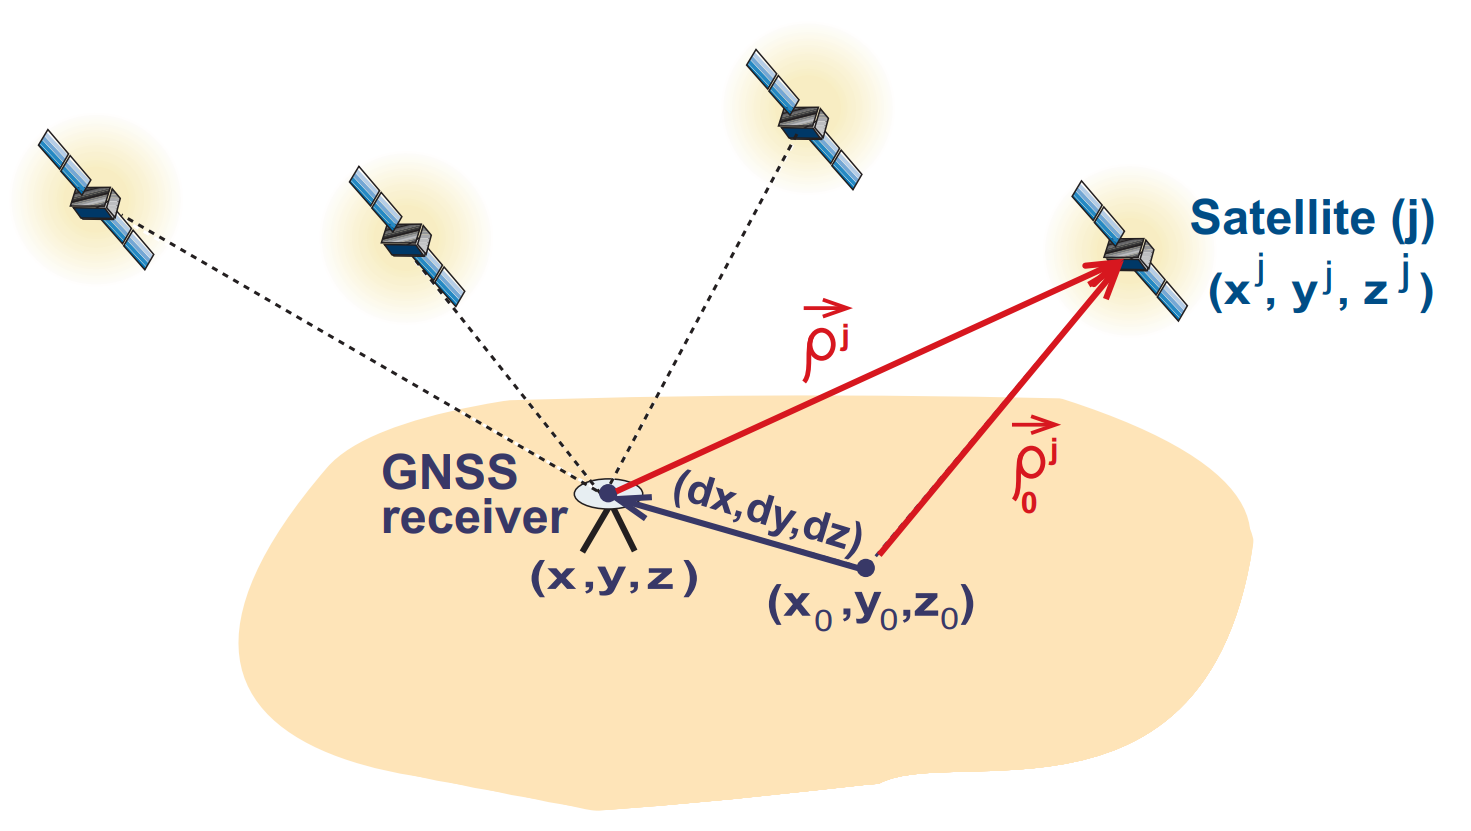
\includegraphics[scale=0.27]{sources/Figures/GNSS_Scheme.png}
        \caption{GNSS Schematic}
        \label{fig:radio magnetic}
\end{figure}


Satellites transmit their positions through "Code" and "Carrier"  \vartext{P_{1}-P_{2}} and \vartext{L_{1}-L_{2}} signals respectively, which contain orbital and time information (\vartext{L1 = 1575.42 MHz} and \vartext{L_{2} = 1227.6 MHz}). The receiver calculates its geographical location by comparing the transmission and reception times of signals received from different satellites. However, the codes must be designed to avoid errors caused by factors such as SNR \fnote{SNR} reduction due to the ionosphere and other electronic losses.

\section{Geometric Range}

To mitigate these errors, filters are employed like the Kalman filter. The Pseudorange-Based Algorithm is used to compute the position, which involves calculating the Euclidean distance from the receiver to each satellite while accounting for noise and time offsets. 

The geometric range $\rho_{rcv}^{sat}$ is computed using the Euclidean distance (see references \citeblue{subirana2013gnss} and \citeblue{HernandezEtAl_GPSDataProcessing}).

\begin{equation}\label{Geometric Range}
    \rho_{rcv}^{sat} = \mid\mid r^{sat}-r_{rcv} \mid\mid = 
\sqrt{\left(x^{sat}-x_{rcv}\right)^{2}+\left(y^{sat}-y_{rcv}\right)^{2}+\left(z^{sat}-z_{rcv}\right)^{2}}
\end{equation}

The measurement \vartext{R = c\Delta T} is the pseodurange mentioned before. This distance is called this way because it is not a real Range distance, but the ones generated by losses due to noise due to atmospheric, electronic and multipath factors are added to the geometric range.

\section{Pseudorange}
For a reference time scale $T$ and using the code $P$ for the frequency signal $f$, the pseudorange for the satellite and receiver is as follows:

\begin{equation}\label{Simple Pseudorange}
    R_{P_{f}} = c\left[t_{rcv}\left(T_{2}\right)-t^{sat} \left(T_{}\right)\right]
\end{equation}

where: $c$ is the speed of light in vacuum, $t_{rcv}\left(T_{2}\right)$ is the time of signal reception, and $t^{sat} \left(T_{}\right)$ the of signal transmission. The time of reception is measured by the receiver clock and the transmission time is measured by the satellite clock.


Then, the pseudorange \vartext{R_{P_{f}}} obtained by the receiver that includes the \vartext{\rho} geometric range between the receiver and the satellite including clock offsets including relativistic effects \vartext{dt_{rcv}} and \vartext{dt^{sat}} and the other terms due to the signal propagation, like ionosphere frequency-dependent delay \vartext{\alpha STEC}\fnote{STEC}, troposphere delay \vartext{Tr}, instrumental frequency and code-dependent delays \vartext{K_{P_{f,rcv}}} and \vartext{K_{P_{f}}^{sat}, receiver \ noise \ \epsilon _{P_{f}}} and multipath effects \vartext{M_{P_{f}}}.



\begin{equation}\label{Pseudorange}
    R_{P_{f}} = \rho + c \left( dt_{rcv} - dt^{sat} \right) + Tr + \alpha STEC + K_{P_{f,rcv}} - K_{P_{f}}^{sat} + M_{P_{f}} + \epsilon _{P_{f}}
\end{equation}


where, \vartext{\alpha_{f} = \frac{40.3}{f^2}10^{16} \ m_{(signal \ delay \ at \ frequency \  f)}/TECU} and \vartext{1 \ TECU = 10^{16}e^{-}/m^{2}}\footnote{\ac{TECU}}.\\


\begin{figure}[H]
        \centering
        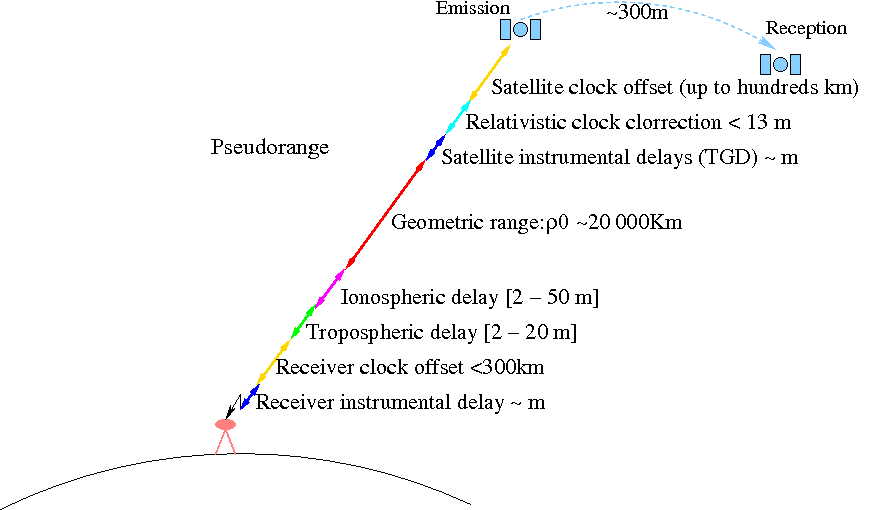
\includegraphics[scale=0.4]{sources/Figures/ranges.png}
        \caption{Pseudorange measurement content \citeblue{GNSSmeasurement}}
        \label{fig:Pseudorange measurement content}
\end{figure}


This is a simple reminder of the different equations that are used to calculate the distances of a receiver with respect to each one of the satellites, being necessary as a minimum of at least 4 satellites (for the precise positioning pointing 5 satellites are needed)so that the receiver can compute the three Cartesian components of the space and time. Otherwise, with more satellites, the precision increases but also the noise of the signal due to the superposition of radio waves.

For a \ac{PPP} a linear model is used following the same procedure as with the \ac{SPP}.




\chapter{Tutorial 2}

\section{Exercise 1: Zenith Troposphere Delay estimation}


Questions:
\begin{enumerate}
\item What is the level of discrepancy between the estimated ZTD and the accurate IGS determination?
\item What is the variation of ZTD in 24 hours due to the wet content?
\item What is the proportion of wet component compared with the dry (or hydrostatic) component?
\end{enumerate}


First of all, to make the labs, a Debian SO has been used. Introducing the following command $lsb_release -a$ we obtain the following output:\\


\begin{figure}[h]
    \centering
    \begin{minted}[fontsize=\footnotesize, bgcolor=bg, breaklines, tabsize=2, frame=lines, framesep=2mm]{console}
        marc@debian:~$ lsb_release -a
        No LSB modules are available.
        Distributor ID: Debian
        Description:    Debian GNU/Linux 11 (bullseye)
        Release:        11
        Codename:       bullseye
    \end{minted}
    \caption{Random noise signal and its representation using Matplotlib. The data has been extracted and plotted using Python.
    }
    \label{fig:Ejemplo de código de bash}
\end{figure}


\begin{figure}[H]
        \centering
        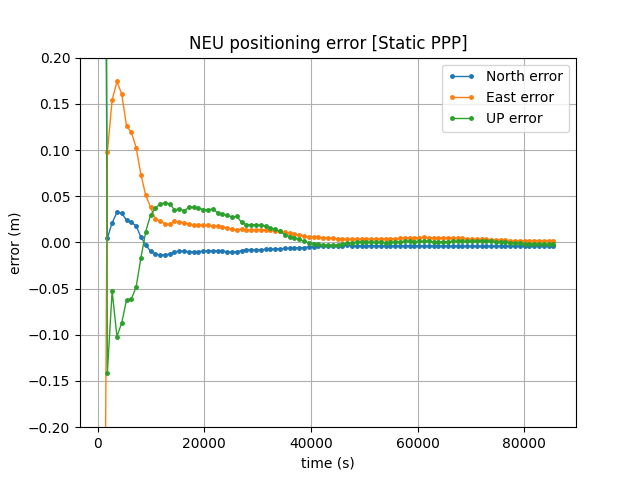
\includegraphics[scale=0.52]{sources/Figures/FIG_2/TUT2_Ex1a.png}
        \caption{}
        \label{fig:}
\end{figure}



\begin{figure}[H]
        \centering
        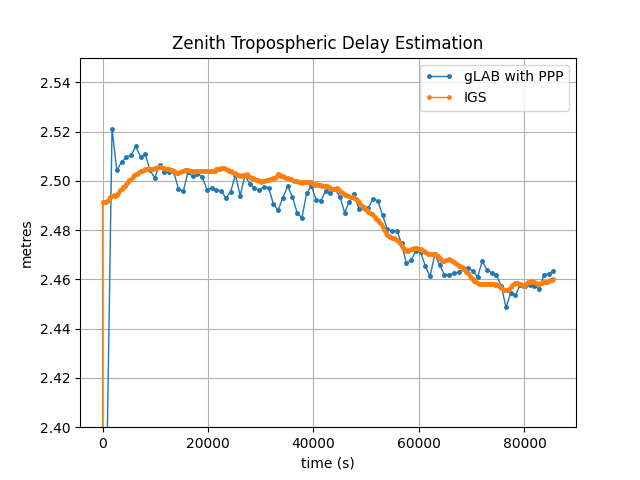
\includegraphics[scale=0.52]{sources/Figures/FIG_2/TUT2_Ex1b.png}
        \caption{}
        \label{fig:}
\end{figure}

\begin{figure}[H]
    \centering
    \begin{subfigure}{0.45\textwidth}
        \centering
        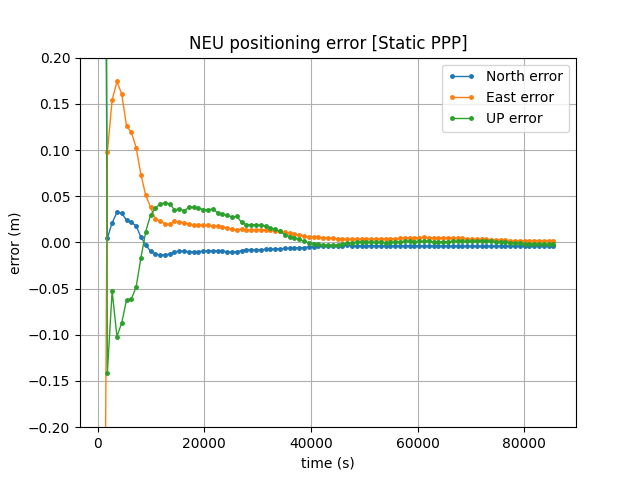
\includegraphics[scale=0.52]{sources/Figures/FIG_2/TUT2_Ex1a.png}
        \caption{}
        \label{fig:subfig1}
    \end{subfigure}
    \hfill
    \begin{subfigure}{0.45\textwidth}
        \centering
        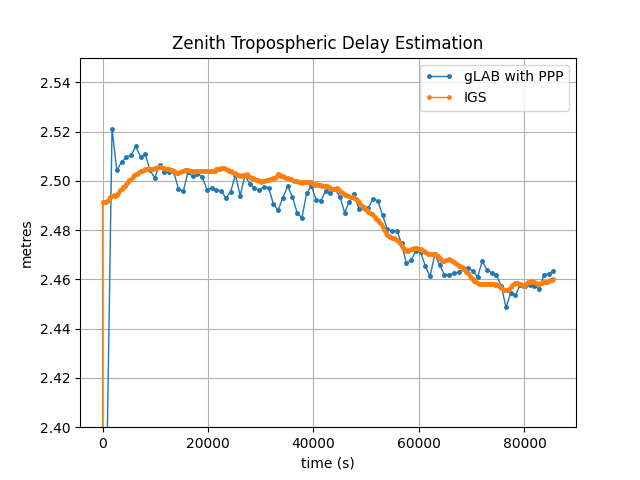
\includegraphics[scale=0.52]{sources/Figures/FIG_2/TUT2_Ex1b.png}
        \caption{}
        \label{fig:subfig2}
    \end{subfigure}
    \caption{}
    \label{fig:dos-figuras-juntas}
\end{figure}
\section{Exercise 2: Ionospheric delay analysis}

Questions:
\begin{enumerate}
\item Justify the expressions used to depict the Ionospheric delay (see slides #16 to #18).
\item Justify the factors of 5.09 and 3.09 used in the P2-L2 and P1-L1 combinations to give the results of L1-L2 delay in metres.
\item Why is the STEC larger at low elevations?
\end{enumerate}


\textcolor{Red}{NOT WORKING}
\begin{figure}[H]
        \centering
        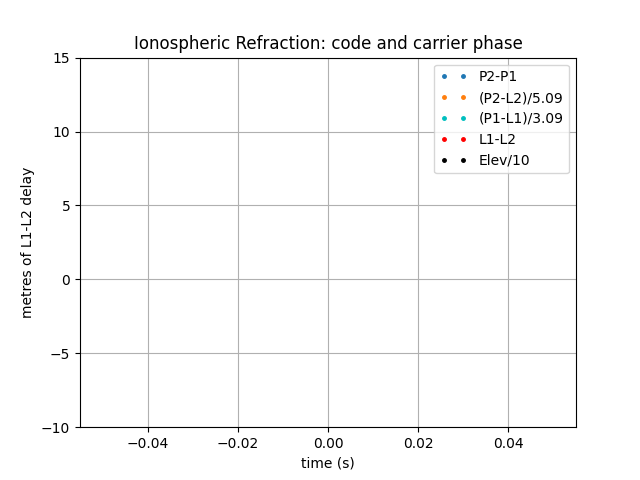
\includegraphics[scale=0.52]{sources/Figures/FIG_2/TUT2_Ex2a.png}
        \caption{}
        \label{fig:}
\end{figure}

\section{Exercise 3.1: Solar Flare October 28, 2003}

Questions:
\begin{enumerate}
\item Why can we associate the sudden increase of TEC seen in the plots with a Solar Flare?
\item What is the STEC variation rate due to the Solar Flare?
\item Can all solar flares be seen in this way?
\end{enumerate}



\begin{figure}[H]
        \centering
        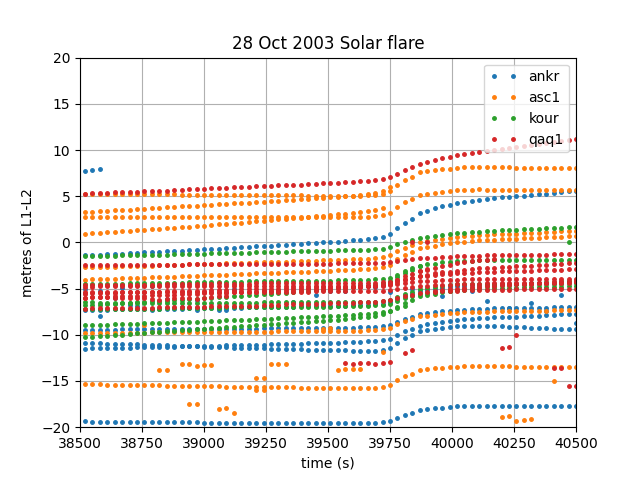
\includegraphics[scale=0.52]{sources/Figures/FIG_2/TUT2_Ex3.1.png}
        \caption{}
        \label{fig:}
\end{figure}
\section{Exercise 3.2: Halloween storm analysis}

Questions:
\begin{enumerate}
\item What is the maximum STEC variation rate seen in the plots?
\item How could we explain the shape of the STECs seen for satellites PRN28 and PRN29?
\end{enumerate}



\begin{figure}[H]
        \centering
        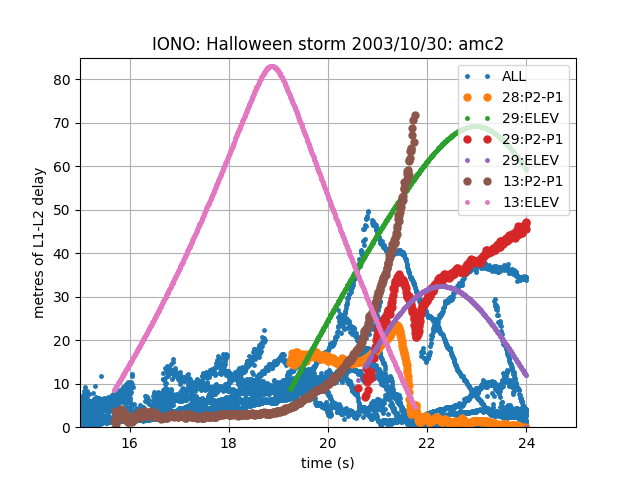
\includegraphics[scale=0.52]{sources/Figures/FIG_2/TUT2_Ex3.2b.png}
        \caption{}
        \label{fig:}
\end{figure}
\section{Ex. 3.3: Halloween storm evolution}

Analyze the ionospheric delays for 6 consecutive days including the Halloween storm:

\begin{enumerate}
\item This is a simple exercise aimed to illustrate the ionospheric delay variation during the Halloween storm. A period of 6 consecutive days (from October 28 to November 2, 2003) are analyzed using measurements collected in the “garl” station in North America.
\item The STEC variations are depicted from the geometry-free combination of codes P2-P1.
\end{enumerate}

Note that:
\begin{equation}\label{Geometry free combination}
    P_{2}-P_{1} = I +K_{21}
\end{equation}


\textcolor{red}{BUG HERE}
\begin{figure}[H]
        \centering
        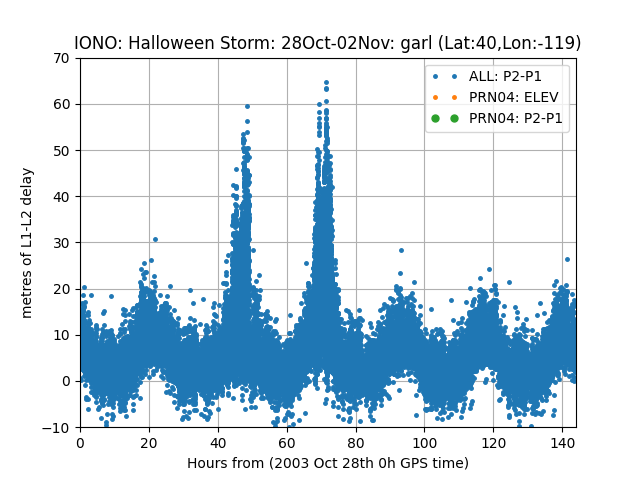
\includegraphics[scale=0.52]{sources/Figures/FIG_2/TUT2_Ex3.3c.png}
        \caption{}
        \label{fig:}
\end{figure}

\textcolor{red}{BUG HERE}
\begin{figure}[H]
        \centering
        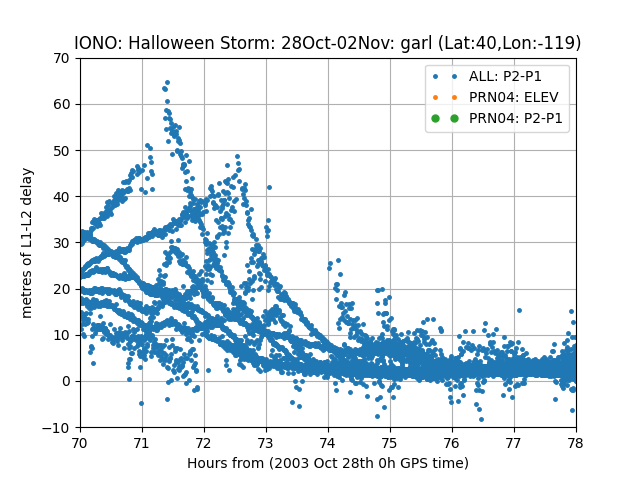
\includegraphics[scale=0.52]{sources/Figures/FIG_2/TUT2_Ex3.3d.png}
        \caption{}
        \label{fig:}
\end{figure}

\begin{enumerate}
\item What is the maximum STEC seen before and after the storm? And during the storm?
\item The STEC of satellite PRN04 shows a flat pattern after time 74 hours which does not change with the elevation. Try to explain this phenomenon.
\end{enumerate}
\section{Exercice 3.4 Single frequency pos. effects}


\textcolor{red}{añadir NEU al glosario}\\
Exercise: Analyze the single frequency positioning solution under the Halloween storm.

The following steps are recommended:
\begin{enumerate}
\item Using files amc23020.03o,brdc3030.03n compute with gLAB the following solutions:
    \begin{enumerate}
        \item Solution with full SPS modeling. Name output file as: gLAB.out
        \item Solution with the ionospheric corrections disabled: gLAB1.out
        \item Solution with the 2-freq. Ionosphere-free code (PC): gLAB2.out
    \end{enumerate}
\item Plot results
\end{enumerate}

\begin{figure}[H]
        \centering
        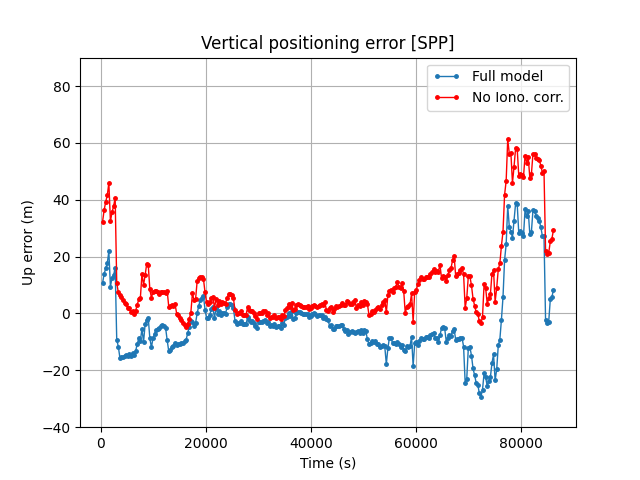
\includegraphics[scale=0.52]{sources/Figures/FIG_2/TUT2_Ex3.4.2c.png}
        \caption{NEU SPP full model with (Klobuchar)}
        \label{fig:NEU SPP full model with (Klobuchar)}
\end{figure}


\begin{figure}[H]
        \centering
        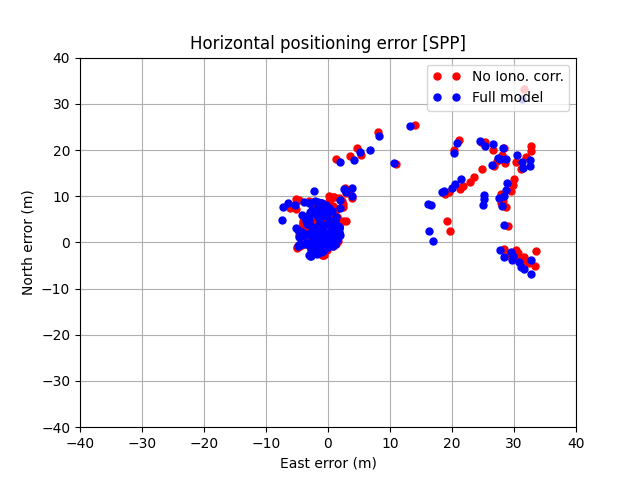
\includegraphics[scale=0.52]{sources/Figures/FIG_2/TUT2_Ex3.4.2d.png}
        \caption{}
        \label{}
\end{figure}


\begin{figure}[H]
        \centering
        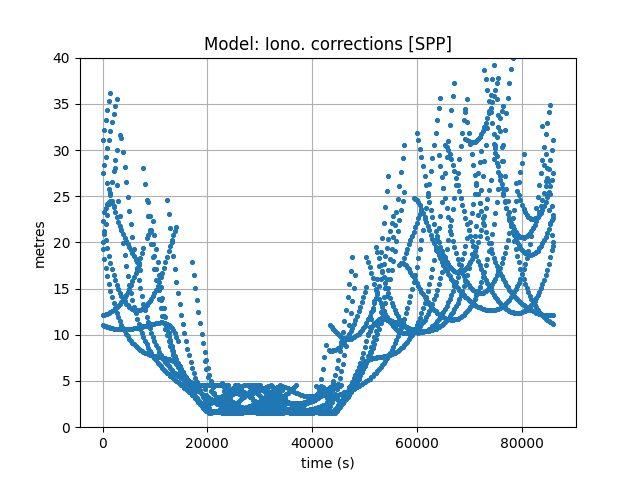
\includegraphics[scale=0.52]{sources/Figures/FIG_2/TUT2_Ex3.4.2e.png}
        \caption{}
        \label{}
\end{figure}


\begin{figure}[H]
        \centering
        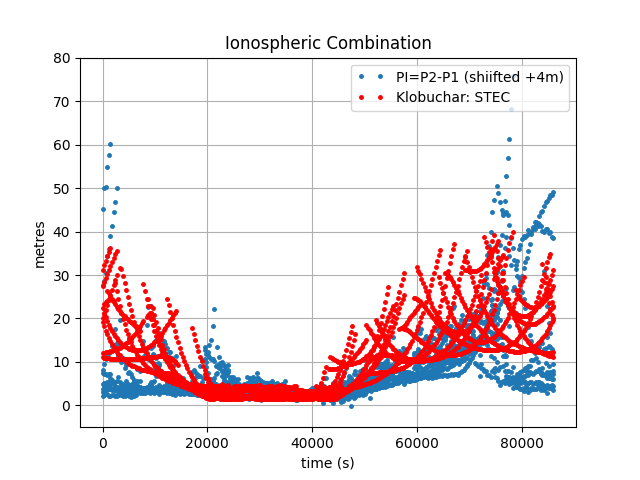
\includegraphics[scale=0.52]{sources/Figures/FIG_2/TUT2_Ex3.4.2f.png}
        \caption{}
        \label{}
\end{figure}
\section{Exercise 4. Code multipath}
The code multipath can be seen by plotting the difference of code and carrier
ionosphere-free combinations (PC-LC). The evolution of this difference can be
followed with a sampling rate of 1 Hz. Due to its geometric nature, the effect
of multipath repeats with the receiver-satellite geometry.\\

The RINEX files \textbf{UPC33600.08N}, \textbf{UPC33610.08N}, UPC33620.08N contain
observations at 1 Hz collected by a GPS receiver with fixed coordinates over
the same period of time on three consecutive days. The corresponding
navigation files are \textbf{BRD3600.08N}, \textbf{BRD3610.08N}, \textbf{BRD3620.08N}.\\

Using gLAB, read the RINEX files, plot the combination PC-LC and identify
the effect of multipath. Analyse the measurements of satellites PRN20 and
PRN25 in the time interval 67000 < t < 68000s. Include the satellite's
elevation in the plots.\\

\subsection{Exercise 4.1 PC Code multipath}
Complete the following steps to depict the noise and multipath in the PC combination:
\begin{enumerate}
        \item Read the RINEX files, execute:
        \begin{figure}[H]
            \centering
            \begin{minted}[fontsize=\footnotesize, bgcolor=bg, breaklines, tabsize=2, frame=lines, framesep=2mm]{console}
            gLAB linux -input:cfg meas.cfg -input:obs UPC33600.08 -input:nav BRD3600.08N > upc3360.meas 
            \end{minted}
            \caption{}
            \label{}
        \end{figure}
        
        \item Verify the following field contents in the generated file upc3360.meas and others:
        
        \begin{figure}[H]
            \centering
            \begin{minted}[fontsize=\footnotesize, bgcolor=bg, breaklines, tabsize=2, frame=lines, framesep=2mm]{python}
            [Id YY Doy sec GPS PRN el Az N. list C1C L1C C1P L1P C2P L2P]
            [1 2 3 4 5 6 x x 9 10 11 xx 13 14 15 16 ]
            \end{minted}
            \caption{}
            \label{}
        \end{figure}

                
        \item Compute the difference of code and carrier ionosphere-free combinations: (i.e. apply next equation) :
\end{enumerate}
    



\begin{equation}\label{Pcode_iono-free}
P_{C} = \frac{f_{1}^{2}P_{1}-f_{2}^{2}P_{2}}{f_{1}^{2}-f_{2}^{2}}
=
\frac{\gamma P_{1}-P_{2}}{\gamma - 1}
\end{equation}

\begin{equation}\label{Carrier_iono-free}
L_{C} = \frac{f_{1}^{2}P_{1}-f_{2}^{2}P_{2}}{f_{1}^{2}-f_{2}^{2}}
=
\frac{\gamma L_{1}-L_{2}}{\gamma - 1}
\end{equation}

Where:

\begin{equation}\label{Pcode_iono-free}
M_{P_{C}} = P_{C}-L_{C}
\end{equation}

\begin{figure}[H]
            \centering
            \begin{minted}[fontsize=\footnotesize, bgcolor=bg, breaklines, tabsize=2, frame=lines, framesep=2mm]{console}
            gawk 'BEGIN{g12=(154/120)**2}{if ($4>66000 && $4<69000)
            print $6,$4,(g12*$13-$15)/(g12-1)-(g12*$14-$16)/(g12-1),$7}' upc3360.meas > upc3360.LcPc
            \end{minted}
            \caption{}
            \label{}
\end{figure}

\textbf{\textcolor{Blue}{(Similarly for the other two files upc3361.meas and upc3362.meas.)}}

Plot the results:
\begin{figure}[H]
            \centering
            \begin{minted}[fontsize=\footnotesize, bgcolor=bg, breaklines, tabsize=2, frame=lines, framesep=2mm]{console}
            graph.py -f upc3360.LcPc -c '($1==20)' -x2 -y3 -s- -l "DoY 360"
                -f upc3361.LcPc -c '($1==20)' -x2 -y3 -s- -l "DoY 361"
                -f upc3362.LcPc -c '($1==20)' -x2 -y3 -s- -l "DoY 362"
                -f upc3360.LcPc -c '($1==20)' -x2 -y4 -l "Elev (deg.)"
            \end{minted}
            \caption{}
            \label{}
\end{figure}

Repeat the same plots, but shift the plot of the second day by 3m 56s = 236s and the third day by 2x(3m 56s) = 472s

\begin{figure}[H]
            \centering
            \begin{minted}[fontsize=\footnotesize, bgcolor=bg, breaklines, tabsize=2, frame=lines, framesep=2mm]{console}
            graph.py -f upc3360.LcPc -c '($1==20)' -x2 -y3 -s- -l "DoY 360"
                -f upc3361.LcPc -c '($1==20)' -x'($2+236)' -y3 -s- -l "DoY 361"
                -f upc3362.LcPc -c '($1==20)' -x'($2+472)' -y3 -s- -l "DoY 362"
                -f upc3360.LcPc -c '($1==20)' -x2 -y4 -l "Elev (deg.)"
            \end{minted}
            \caption{}
            \label{}
\end{figure}



\begin{figure}[H]
    \centering
    \begin{subfigure}{0.45\textwidth}
        \centering
        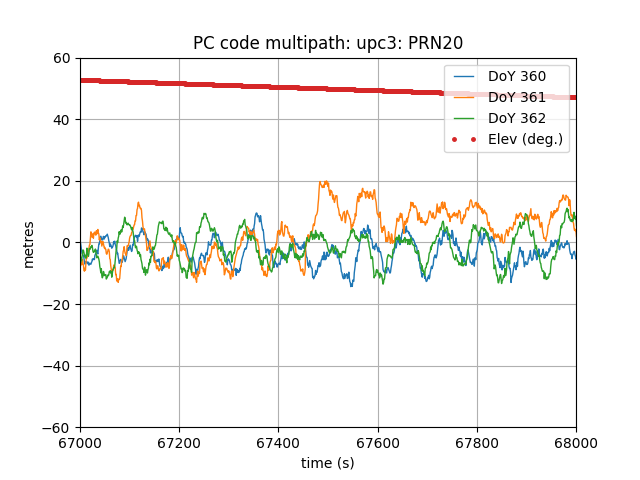
\includegraphics[scale=0.52]{sources/Figures/FIG_2/TUT2_Ex4.1a.png}
        \caption{}
        \label{fig:subfig1}
    \end{subfigure}
    \hfill
    \begin{subfigure}{0.45\textwidth}
        \centering
        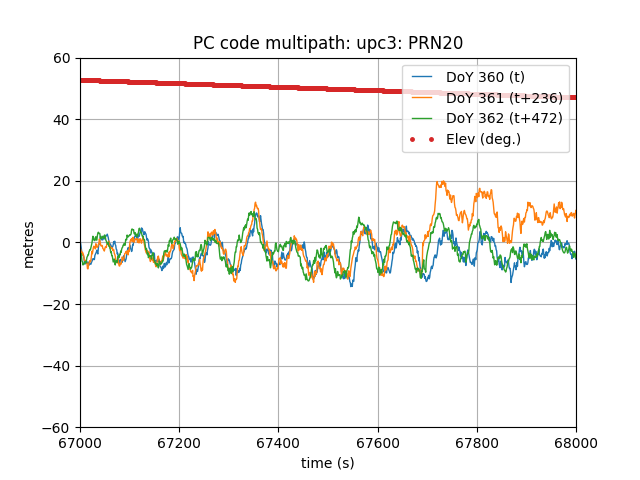
\includegraphics[scale=0.52]{sources/Figures/FIG_2/TUT2_Ex4.1b.png}
        \caption{}
        \label{fig:subfig2}
    \end{subfigure}
    \caption{}
    \label{fig:dos-figuras-juntas}
\end{figure}


\begin{figure}[H]
        \centering
        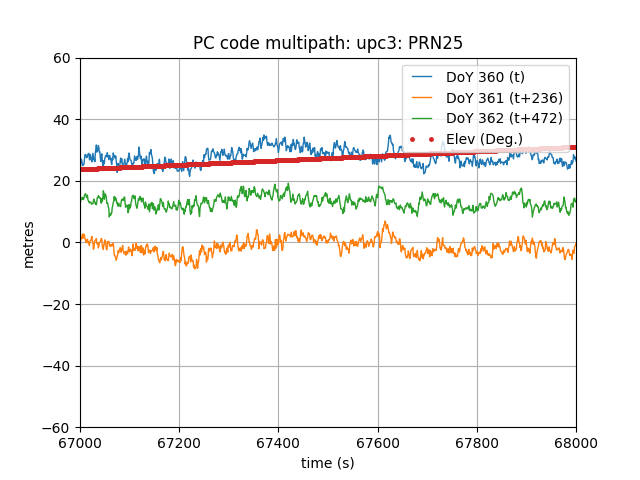
\includegraphics[scale=0.52]{sources/Figures/FIG_2/TUT2_Ex4.1.5.png}
        \caption{}
        \label{}
\end{figure}
\usepackage{subcaption}







\begin{itemize}
    \item What is the reason for the observed 3m 56s displacement between the graphs for two consecutive days?
    \item Repeat the previous plot for the satellite PRN25 and compare results.
\end{itemize}

\textcolor{Green}{OPTIONAL: Repeat the multipath analysis of the previous exercise using
files htv13450.04o, htv13460.04o, htv13470.04o collected by the
permanent receiver HTV1, and files galb3450.04o, galb13460.04o,
galb13470.04o collected by the permanent receiver GALB. The associated
broadcast orbit files are brdc3450.04n, brdc3460.04n, brdc3470.04n.}



\subsection{Exercise 4.2. Melbourne-Wübbena multipath}

Complete the following steps to depict the noise and multipath in the Melbourne Wübbena combination:

\begin{equation}\label{Pcode_Wübbena}
P_{N} = \frac{f_{1}P_{1}+f_{2}P_{2}}{f_{1}+f_{2}}
=
\frac{\sqrt{\gamma} P_{1}-P_{2}}{\sqrt{\gamma} - 1}
\end{equation}

\begin{equation}\label{Carrier_Wübbena}
L_{W} = \frac{f_{1}L_{1}-f_{2}L_{2}}{f_{1}-f_{2}}
=
\frac{\sqrt{\gamma} L_{1}-L_{2}}{\sqrt{\gamma} - 1}
\end{equation}

Where:

\begin{equation}\label{Pcode_Wübbena}
M_{MW} = P_{N}-L_{W}
\end{equation}


Execute (in a single line):\\

\begin{figure}[H]
            \centering
            \begin{minted}[fontsize=\footnotesize, bgcolor=bg, breaklines, tabsize=2, frame=lines, framesep=2mm]{console}
            gawk 'BEGIN{s12=154/120}{print $6,$4,(s12*$14-$16)/(s12-1)-(s12*$13+$15)/(s12+1),$7}' galb3450.meas > galb3450.MW
            \end{minted}
            \caption{}
            \label{}
\end{figure}


\textbf{\textcolor{Blue}{(Similarly for the other files)}}\\

And plot results.





\subsection{Exercise 4.3. C1 code multipath}
The C1 code multipath and receiver noise can be depicted using the following combination (that removes all frequency dependent and not dependent terms):

\begin{equation}\label{}
M_{C_{1}} =C_{1}-L_{1}-2\alpha\left(L_{1}-L_{2}\right) ; \ \ \ \ \ \ \alpha = \frac{f_{2}^{2}}{f_{1}^{2}-f_{2}^{2}} = \frac{1}{\gamma -1} = 1.545 ; \ \ \ \ \ \ \gamma = \left(\frac{77}{60}\right)^{2}
\end{equation}


\begin{itemize}
    \item \textbf{\textcolor{Blue}{Generate the “meas” file: Select, for instance, PRN03}}
    \begin{figure}[H]
            \centering
            \begin{minted}[fontsize=\footnotesize, bgcolor=bg, breaklines, tabsize=2, frame=lines, framesep=2mm]{console}
            gLAB_linux -input:cfg meas.cfg -input:obs UPC33510.08O|gawk '{if ($6==03)print $0}'>upc3.meas
            \end{minted}
            \caption{}
            \label{}
    \end{figure}
    \begin{figure}[H]
            \centering
            \begin{minted}[fontsize=\footnotesize, bgcolor=bg, breaklines, tabsize=2, frame=lines, framesep=2mm]{python}
            [Id YY Doy sec GPS PRN el Az N. list C1C L1C C1P L1P C2P L2P]
            [1 2 3 4 5 6 7 8 9 10 11 12 13 14 15 16 ]
            \end{minted}
            \caption{}
            \label{}
    \end{figure}

    
    \item \textbf{\textcolor{Blue}{Using previous expression, compute the C1 multipath and code noise:}}
    \begin{figure}[H]
            \centering
            \begin{minted}[fontsize=\footnotesize, bgcolor=bg, breaklines, tabsize=2, frame=lines, framesep=2mm]{console}
            gawk '{print $4,$11-$14-3.09*($14-$16)-21.3}' upc3.meas> upc3.C1
            \end{minted}
            \caption{}
            \label{}
    \end{figure}


    
    \item \textbf{\textcolor{Blue}{Plot results for PRN03:}}
    \begin{figure}[H]
            \centering
            \begin{minted}[fontsize=\footnotesize, bgcolor=bg, breaklines, tabsize=2, frame=lines, framesep=2mm]{console}
            graph.py -f upc3.C1 -s- --l "C1 Raw" --xn 35000 --xx 40000  --yn -5 --yx 5 --xl "time (s)" --yl "meters"  -t "PRN03, C1 Raw measurement noise and multipath"
            \end{minted}
            \caption{}
            \label{}
    \end{figure}
\end{itemize}





\printbibliography

\clearpage  
\newpage

\appendix
\chapter{Acronyms}
\begin{acronym}
\acro{ESA}{European Space Agency}
\acro{GPS}{Global Positioning System}
\acro{NASA}{National Aeronautics and Space Administration}
\acro{PPP}{Precise Point Positioning}
\acro{SNR}{Signal to Noise Ratio}
\acro{SPP}{Standard Point Positioning}
\acro{STEC}{Slant Total Electron Content}
\acro{TECU}{Total Electron Content Unit}
\end{acronym}




\clearpage  
\newpage

\end{document}
